\documentclass[submission,copyright,creativecommons]{eptcs}
\providecommand{\event}{TeaseLP} % Name of the event you are submitting to

\usepackage{amsmath}
\usepackage{amssymb}

\usepackage{breakurl}             % Not needed if you use pdflatex only.
\usepackage{underscore}           % Only needed if you use pdflatex.
\usepackage{graphicx}
\usepackage{booktabs}
\usepackage{cleveref}


\hypersetup{hidelinks}

\title{Accelerating Program Synthesis in miniKanren}
\author{Robert Zinkov
\institute{University of Oxford \\
Oxford, UK}
\email{zinkov@robots.ox.ac.uk}
\and
Michael Ballantyne
\institute{Northeastern University\\
Boston, MA, USA}
\email{ballantyne.m@northeastern.edu}
\and
Gregory L. Rosenblatt
\institute{University of Alabama at Birmingham\\
Birmingham, AL, USA}
\email{gregr@uab.edu}
\and
William E. Byrd
\institute{University of Alabama at Birmingham\\
Birmingham, AL, USA}
\email{webyrd@uab.edu}
}
\def\titlerunning{Speeding up Search for Logic Programs}
\def\authorrunning{R. Zinkov et al.}
\begin{document}
\maketitle

\begin{abstract}
  While many logic programming systems like miniKanren are highly
  expressive, they suffer from long and unpredictable running times.
  The challenge comes from the search algorithm being usually an
  uninformed search. Through the domain of program synthesis
  we show that it possible to greatly speedup this search by guiding
  it using example programs.
  
\end{abstract}

\section{Introduction}

In the miniKanren\cite{byrd2017unified} programming language, we often
pose relations in a compostional manner, where more complicated
relations are defined in terms of simpler relations. These simple
relations include $\equiv$ defining constraints and $\textbf{cond}^e$
for defining a logical disjunction over clauses. In $\textbf{cond}^e$
we have to make a decision over the order we explore each of the
clauses. If we pick well, we quickly find an answer that satisfies our
constraints. If we pick less well, we hope we quickly find a
constraint violation and backtrack immediately. If we pick badly, it
could take a long while to get an answer at all.

Now, it can feel like there might an optimal way to arrange the
clauses but this runs into several problems. Firstly, our instincts of
which clause to try first are in many settings not obvious or intuitive. Secondly,
what ordering might make sense in the absence of constraints might not make
sense in their presence. But most importantly, the best ordering is highly
contextual and when dealing with relations which are recursively-defined
the best ordering could be different from call to call.

To deal with this issue we take a cue from existing machine learning
work\cite{zaremba2014learning,lee2018accelerating} and learn a search
heuristic to guide the search. More specifically, as outlined in
\Cref{fig:overview} we learn a probabilistic model to choose which
clause to pick given the context the choices exist within.

As an example consider a grammar like the lambda-calculus. Suppose we
are trying to generate the operand $e_2$ of a function application. We
can use the context of being the operand in the expression to decide
what program we generate. To decide what expressions to generate we
might look at a set of example programs and count in the operand
position what is most likely a symbol, a function abstraction, or a
function application. Then we should bias our search to look more like
example programs. Particularly, if we are trying to generate programs
that resemble a given set of example programs.

\begin{figure}
\begin{eqnarray*}
  e & := & x \; | \; (e_1 \; e_2) \; | \; (\lambda \; (x) \; e_1) \\
\end{eqnarray*}
\caption{Example grammar}
\end{figure}

This can be reasonable for small grammars like the lambda calculus, but
what should we do if we end up in a context we have never seen before?
In that case, we don't want to say an expression shouldn't be generated
even if we don't possess an example. So we assume every choice was seen
at least once or what is sometimes called Laplacian smoothing.

We train this model by collecting a dataset of (context, choice)
pairs. These are created in a domain-specific way from example
programs that be converted into these (context, choice) pairs in an
entirely offline manner. For each pair we count what choices were made
per context. These counts are then saved into a table that our
implementation of $\textbf{cond}^e$ accesses selecting clauses from
most to least probable, thus guaranteeing the search stays complete.

\begin{figure}[htb!]
\centering
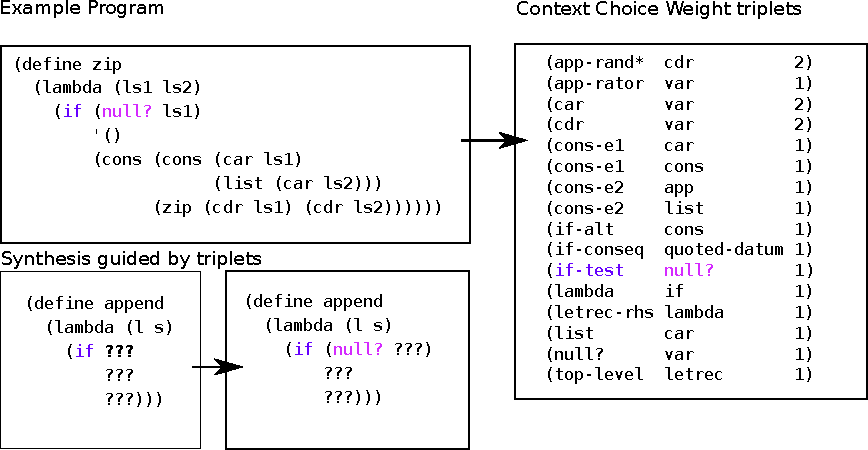
\includegraphics[scale=1.0]{drawing.pdf}
\caption{Overview of the system}
\label{fig:overview}
\end{figure}


\section{Experiments}

We show a preliminary evaluation in the table below. The following
results come from trying to complete a program synthesis
task. Synthesis is defined as satisfying a query in a relational
interpreter written in miniKanren. We first try to synthesise programs
where an expert chooses the ordering of the different rules in the
grammar, and then with our method where we use the probabilities of
a learned model to select the grammar rule.

The interpreter is for a subset of the Scheme language, and we are
thus able to train using a collection of programs sourced from the
Little Schemer and the Seasoned Schemer.

\begin{table}[ht]
\centering
\caption{Times for completing synthesis test in seconds}
\begin{tabular}[t]{lcc}
\toprule
Program&Expert ordering&$n$-gram directed ordering\\
\midrule
append&0.9809&0.5906\\
reverse&--&0.0115\\
rember&0.0103&0.007\\
foldr&2.3881&0.0064\\
\bottomrule
\end{tabular}
\end{table}

We show that in isolation this optimisation yields
significant speedups on several programs. For some programs, like
reverse, the original program did not find a solution even when given
several minutes.

\section{Future Work}

The present method is highly specialised to the program synthesis task
of Barliman, but there is a significant possibility that if we had a
dataset of queries and query answers, we could generalise our results
for miniKanren programs in general.

%\nocite{*}
\bibliographystyle{eptcs}
\bibliography{paper}
\end{document}
